\documentclass[11pt]{article}
\usepackage[margin=1in]{geometry}
\usepackage[T1]{fontenc}
\usepackage{lmodern}
\usepackage{amsmath,amssymb,amsthm}
\usepackage{booktabs}
\usepackage{tikz}
\usetikzlibrary{arrows.meta,positioning}
\usepackage[hidelinks]{hyperref}
\usepackage{enumitem}
\setlist{nosep,leftmargin=*}
\newtheorem*{conj}{Conjecture}
\newtheorem*{thm}{Theorem}
\newcommand{\lean}[1]{\texttt{#1}}
\emergencystretch=3em
\title{Where We Are: The Lucas Conjecture,\\ Frege vs.\ Extended Frege, and an Honest Map}
\author{Working notes for Vasily Shablov, by Claude}
\date{October 2026}
\begin{document}
\maketitle

\section{The short version}

You are right that the paper reads as applied. About two thirds of its pages are a
measurement of Mathlib, and the theory is spread across it. The theoretical core is real
but small. Here is the honest inventory.

\begin{center}\small
\begin{tabular}{p{0.52\linewidth}p{0.18\linewidth}p{0.2\linewidth}}
\toprule
Result & Status & Depth \\
\midrule
Value of one name: $(k-1)(b-1)-1$ & proved (Lean) & elementary \\
Unfolding $\le 2^i$, $d$-bonacci sharp bound & proved (Lean) & easy--moderate \\
Exact value $(o-1)(W-1)-1$ in any library & proved (Lean) & moderate, new \\
Rank-one (Schur) updates of naming & proved (Lean) & moderate, new \\
Concepts are substitutes (submodularity) & proved (Lean) & moderate, likely new \\
Bounded readers see complements & proved (Lean) & small example \\
Speed limit $\le 28\cdot(5/4)^C$ & proved (Lean) & moderate, likely new \\
Lucas library reaches $2L_m-2$ & proved (Lean) & construction \\
\textbf{Lucas conjecture} (max is exactly $2L_m-2$) & \textbf{open}; verified $m\le15$ & the real theorem to prove \\
Frege vs.\ Extended Frege & \textbf{open, famous}; untouched & far beyond us for now \\
Mathlib measurements (growth law, taste AUCs, glue) & empirical & applied \\
\bottomrule
\end{tabular}
\end{center}

\noindent \emph{Likely new} means a literature search turned up nothing; a specialist
should still check. The rest of this note explains the two names you asked about, says
plainly where the theory stands, and suggests how to turn this into a genuinely
theoretical paper.

\section{The Lucas conjecture, from scratch}

\subsection{The game}

You build a library one result at a time. Each new result either:
\begin{itemize}
\item is a \emph{leaf}: it cites nothing; or
\item cites some \emph{distinct} earlier results.
\end{itemize}

\paragraph{Price.} Writing a result costs $1$ symbol for itself plus $1$ symbol per
citation. The \emph{named cost} $C$ is the total over all results.

\paragraph{Payoff.} The \emph{unfolded size} of a result is what you would have to write
if every citation were replaced by a full copy of the cited proof, recursively:
\[
u(\text{result}) = 1 + \sum_{\text{cited results } j} u(j).
\]
Equivalently, $u$ counts the paths starting at that result in the citation graph.

\paragraph{Question.} With $C$ symbols of named writing, how large can an unfolded
size be? In other words, how much mathematics can a library of size $C$ \emph{stand for}?

\subsection{Small examples}

\begin{itemize}
\item \textbf{Cost 6.} Leaf $a$ (cost 1, $u=1$); $b$ cites $a$ (cost 2, $u=2$); $c$ cites
  $a,b$ (cost 3, $u=1+1+2=4$). Best possible: $4$.
\item \textbf{Cost 12: the Lucas library for $m=4$.} Each column below is one result.
\end{itemize}
\begin{center}\small
\begin{tabular}{lccccc}
\toprule
result & $r_0$ & $r_1$ & $r_2$ & $r_3$ & $r_4$ \\
\midrule
cites & -- & $r_0$ & $r_1$ & $r_2, r_1$ & $r_3, r_2, r_1$\\
cost & 1 & 2 & 2 & 3 & 4 \\
$u$ & 1 & 2 & 3 & $1+3+2=6$ & $1+6+3+2=12$\\
\bottomrule
\end{tabular}
\end{center}
\noindent The total cost is $12$ and the top result has $u=12$.

\begin{center}
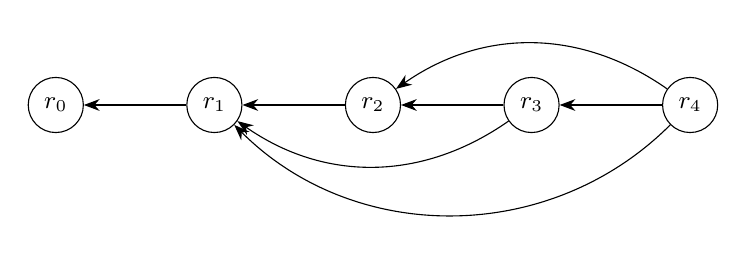
\begin{tikzpicture}[node distance=13mm, every node/.style={circle,draw,minimum size=7mm,font=\small}, >={Stealth[length=2mm]}]
\node (r0) {$r_0$};
\node (r1) [right=of r0] {$r_1$};
\node (r2) [right=of r1] {$r_2$};
\node (r3) [right=of r2] {$r_3$};
\node (r4) [right=of r3] {$r_4$};
\draw[->] (r1) -- (r0);
\draw[->] (r2) -- (r1);
\draw[->] (r3) -- (r2);
\draw[->] (r3) to[bend left=35] (r1);
\draw[->] (r4) -- (r3);
\draw[->] (r4) to[bend right=35] (r2);
\draw[->] (r4) to[bend left=45] (r1);
\end{tikzpicture}

\small Arrows point to cited results. Unfolded size $u(r_4)=12$ = the number of paths
starting at $r_4$.
\end{center}

\paragraph{The general pattern.} Start with a leaf and a short chain, then make every
result cite the two before it. This is the Fibonacci step: it costs $3$ symbols and
multiplies $u$ by about $\varphi\approx1.618$. Finish with one result citing the top
three. At cost $3m$ this gives exactly $2L_m-2$, where the Lucas numbers are
$L=2,1,3,4,7,11,18,29,\ldots$ (each is the sum of the previous two).

\subsection{The conjecture}

\begin{conj}[Lucas law of compression]
For every $m\ge4$, the largest unfolded size achievable with named cost $3m$ is exactly
$2L_m-2$. Consequently, the best possible growth rate is $\varphi^{1/3}\approx1.174$ per
written symbol.
\end{conj}

\noindent In words: no cleverer way of organizing a library beats the Fibonacci pattern.
The golden ratio would be the \emph{speed limit of compression}.

\subsection{What is proved, and what is not}

\paragraph{Proved in Lean.}
\begin{itemize}
\item The Lucas library really does reach $2L_m-2$ at cost $3m$ (\lean{lucasLib\_top},
  \lean{lucasLib\_cost}).
\item \emph{Every} library satisfies $u\le 28\cdot(5/4)^C$ (\lean{ULib.u\_le}).
\end{itemize}
So the true rate lies in the bracket
\[
\varphi^{1/3}\approx 1.174 \;\le\; \text{rate} \;\le\; 1.25.
\]
The trivial bound, which multiplies $(1+\#\text{citations})$ over all results, gives only
$3^{1/3}\approx1.442$.

\paragraph{Checked by computer, not proved.} An exact search confirms the conjecture for
every $m$ from $4$ to $15$. The search is valid because citing the largest available
results is always best, so the state of a library is just the multiset of its sizes. It
allowed up to 9 citations per result for cost up to $39$, and up to 5 citations up to cost
$45$.

\paragraph{Why it is hard: the obstacle we found.} The $5/4$ proof uses a
\emph{potential}: a weighted sum of the largest one, two and three unfolded sizes, shown to
grow by at most $5/4$ per symbol. We proved, by linear-programming duality, that
\emph{no} potential of this linear kind can certify any rate below $1.2198$. So reaching
$\varphi^{1/3}$ needs a genuinely new idea. The culprit is states containing many copies of
the same large value: such a state is expensive to build but cheap to exploit, and linear
potentials cannot account for the cost of building it.

\paragraph{Three plausible routes to a proof.}
\begin{enumerate}
\item \textbf{A nonlinear potential}: a maximum of several linear pieces, one for each
  ``opening move'' followed by Fibonacci. Our numerical attempts suggest the true value
  function needs infinitely many pieces. It might nevertheless have a clean closed form.
\item \textbf{Structural exchange lemmas.} Show directly that an optimal library never
  uses a result with $4$ or more citations, uses single-citation results only at the
  start, and so on. This reduces the problem to the Fibonacci pattern.
\item \textbf{Entropy.} Count paths via the entropy of a random path. The local choice at
  each result (stop, or follow one of its citations) has entropy that may be bounded
  against its cost of $1+d$. This is the classical way golden-ratio bounds get proved.
\end{enumerate}

\paragraph{Why it matters.} It is a clean, self-contained extremal problem: how many paths
can a directed acyclic graph have, given vertices plus edges? It has an unexpected exact
Lucas-number answer, and it says precisely how much a library of concepts can stand for.
The golden ratio also appears as the conjectured answer in a related open problem, the
number of monotone paths on 3-dimensional polytopes (Athanasiadis--De~Loera--Zhang). A full
proof would be a real, citable theorem in extremal combinatorics.

\section{Frege and Extended Frege, from scratch}

\subsection{Proof systems for propositional logic}

\paragraph{Tautologies.} A \emph{tautology} is a formula true under every assignment, for
example $p\lor\lnot p$, or ``if $n+1$ pigeons sit in $n$ holes, two share a hole'' written
in propositional variables.

\paragraph{Proof systems.} A \emph{proof system} is a checkable format for certifying
tautologies. The central question of proof complexity (Cook--Reckhow, 1979): \emph{does
every tautology have a short proof?} If some proof system gave polynomial-size proofs of
all tautologies, then NP $=$ coNP. So showing that every system needs long proofs for some
tautologies is a route toward P $\neq$ NP. Researchers climb a ladder of systems, proving
lower bounds for stronger and stronger ones.

\subsection{Frege}

A \emph{Frege system} is the textbook system: a few axiom schemes plus modus ponens.
\begin{itemize}
\item A proof is a list of formulas, each an axiom or following from earlier ones.
\item The size of a proof is the total number of symbols.
\item Any two Frege systems simulate each other with polynomial overhead, so ``Frege''
  names one robust level of the ladder.
\end{itemize}

\paragraph{Lemmas are free.} A line, once proved, can be reused later, so a Frege proof is
naturally a DAG. Kraj\'i\v{c}ek showed that tree-like Frege proofs, where every reuse is
re-proved, are only polynomially longer. In Frege, reusing lemmas saves at most a
polynomial.

\paragraph{What is known.} Strong (exponential) lower bounds exist for weaker systems such
as resolution and bounded-depth Frege. For full Frege, \emph{no super-polynomial lower
bound is known for any tautology}. This is one of the major open problems of the field.

\subsection{Extended Frege: adding the power to name}

\emph{Extended Frege} (EF) adds one rule, Tseitin's \emph{extension rule}: at any point you
may introduce a \textbf{brand-new variable} $q$ and the axiom
\[
q \leftrightarrow \varphi,
\]
where $\varphi$ is any formula. The variable $q$ must not occur earlier, in $\varphi$, or in
the conclusion. That is all.
\begin{itemize}
\item $q$ is a \textbf{definition}: a name for a possibly huge formula.
\item Afterwards you can write $q$ instead of $\varphi$, and nest definitions inside
  definitions.
\item In complexity terms, Frege reasons with formulas (roughly the class NC$^1$), while
  EF reasons with circuits (roughly polynomial-size circuits, P). Naming is exactly what
  turns a formula into a circuit: it lets a subexpression be shared.
\end{itemize}

\begin{conj}[open: Frege vs.\ Extended Frege]
Is EF super-polynomially stronger than Frege? That is, are there tautologies with
polynomial-size EF proofs but no polynomial-size Frege proofs?
\end{conj}

\noindent Nobody knows. Candidate separating examples have been studied, for instance
tautologies about matrix algebra that have short EF proofs and are hard to handle with
formulas alone. No separation has been proved. Proving one would need, at the very least,
the first super-polynomial Frege lower bound, itself a famous open problem.

\subsection{Why it is \emph{our} question}

Our project asks: \emph{does mathematics need new concepts, or are they only convenient?}
Proof complexity has the sharpest form of that question, at two levels.
\begin{enumerate}
\item \textbf{Naming proved statements (lemmas).} Answered for Frege: at most a polynomial
  saving (Kraj\'i\v{c}ek). Our exponential theorems are about \emph{copying} lemmas, which
  is naive. A clever prover restructures instead of copying. That is why we corrected our
  ``Mathlib does not fit in the universe'' claim.
\item \textbf{Naming new formulas (definitions).} This is exactly Frege versus Extended
  Frege: whether the power to define new concepts can save super-polynomially. It is
  open.
\end{enumerate}

\noindent At the level of higher-order concepts the answer is known and dramatic. G\"odel
(1936) and Boolos (1987) give statements whose first-order proofs are unimaginably long
but which have short proofs once higher-order concepts are allowed. So concepts are
provably essential ``at the top'', and unknown ``at the bottom''.

\paragraph{Our honest relation to it.} We did \textbf{not} make progress on Frege vs.\
EF, and I do not claim any. Our calculus of naming (exact value, rank-one updates,
submodularity) lives in a fixed citation DAG. It prices naming versus copying within one
given proof. It does not let the prover choose a different proof, and that freedom is the
heart of proof complexity. One could try to bridge the gap: define naming over \emph{all}
proofs of a statement and ask how the optimum behaves. That would be a real research
program, not a weekend.

\section{Why the paper feels applied, and how to fix it}

\paragraph{Diagnosis.}
\begin{itemize}
\item The paper grew in the order we worked: measurement first, theory later.
\item Its first theorems are elementary: $(k-1)(b-1)-1$ is one line of algebra.
\item The two genuinely theoretical results, the calculus of naming and the speed limit,
  arrived last and sit in the middle of empirical sections.
\item The strongest open problem, the Lucas conjecture, is unresolved, so the paper has
  no headline theorem.
\end{itemize}

\paragraph{Proposal: split into two papers.}
\begin{enumerate}
\item \textbf{A theory paper}, roughly ``A calculus of naming and the speed limit of
  compression''.
  \begin{itemize}
  \item \emph{Model:} libraries as DAGs, namings as vertex sets.
  \item \emph{Exact value and the elimination view:} rank-one updates, Schur complements.
  \item \emph{Submodularity, and complementarity for bounded readers.}
  \item \emph{Complexity of optimal naming.} New target: prove NP-hardness, or find a
    polynomial algorithm for special classes such as trees and bounded treewidth.
  \item \emph{The speed limit.} The proved bracket and the Lucas conjecture, ideally
    proved.
  \item \emph{Variants.} Citations with multiplicity, where the limit should move to
    $3^{1/3}$, and variable sizes.
  \end{itemize}
  No data. Mathlib appears only as one motivating paragraph.
\item \textbf{An empirical paper}: the measurement of Mathlib, the two axes of taste, the
  glue layer and the law of abbreviation, with the theory paper cited for the model.
\end{enumerate}

\paragraph{What would make the theory paper strong.} In order of value:
\begin{enumerate}
\item a proof of the Lucas conjecture, or at least of the rate $\varphi^{1/3}$;
\item a hardness theorem for optimal naming (or an algorithm);
\item a sharp speed limit for the multiplicity variant;
\item a clean statement linking capacity-bounded comprehension to the speed limit: how
  much a reader of capacity $B$ can understand with a library of size $C$.
\end{enumerate}
Items 2--4 look feasible with focused work. Item 1 is a genuine research problem: it
could take one good idea, or much longer.

\section{One-paragraph summary}

We turned ``what makes a mathematical idea fruitful?'' into mathematics.
\begin{itemize}
\item \textbf{The exact theory.} A concept is a compression. Its exact value is the
  product of how often it is needed and how much it hides. Naming acts like Gaussian
  elimination run backwards. Concepts are substitutes for compression and complements for
  bounded understanding.
\item \textbf{The speed limit.} Compression has a provable speed limit between
  $\varphi^{1/3}$ and $5/4$ per symbol. The \textbf{Lucas conjecture} says it is exactly
  the golden one.
\item \textbf{The deep form.} The deepest version of ``are concepts necessary?'' is the
  open \textbf{Frege vs.\ Extended Frege} problem. We explain it but did not advance it.
\item \textbf{Next.} The theory deserves its own paper; the Mathlib measurements deserve
  another.
\end{itemize}

\end{document}
